\section{VIAJES}
\subsection{Gráfico de dependencias}
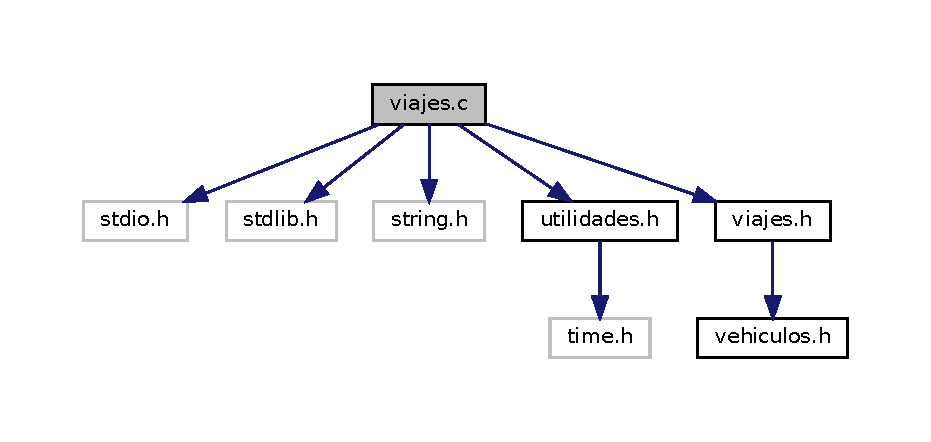
\includegraphics[width=\textwidth, angle=0]{dep/viajes_include.pdf}
\subsection{Estructura de Datos}
\begin{itemize}
    \item \funrf{struct Viajes}{struct:viajes}
    \item \funrf{struct Pasos}{struct:pasos}
    \item \funrf{struct vViajes}{struct:viajespasos}
\end{itemize}
\subsection{Funciones}
\begin{itemize}
    \item \funrf{Viajes* initViajes(int* n)}{initviajes}
    \item \funrf{Pasos* initPasos(int* n)}{initpasos}
    \item \funrf{void publicarViajeUsuario(vViajes* v,vVehiculos* ve,int userId)}{puviuser}
    \item \funrf{void editarViajesUsuario(vViajes* v,vVehiculos* ve,int userId)}{editviuser}
    \item \funrf{void incorporarseViaje(vViajes* v)}{inviuser}
    \item \funrf{void detalleViaje(vViajes* v)}{detallavi}
    \item \funrf{void publicarViajeAdmin(vViajes* v, vVehiculos* ve)}{puviadmin}
    \item \funrf{void eliminarViajesAdmin(vViajes* v)}{delviadmin}
    \item \funrf{void modificarViajesAdmin(vViajes* v,vVehiculos *vve)}{editviadmin}
    \item \funrf{void listarViajesAdmin(vViajes* v)}{listviadmin}
    \item \funrf{void saveViajes(int n,Viajes* viajes)}{savevi}
    \item \funrf{void savePasos(int n,Pasos* pasos)}{savevipa}
    \item \funrf{int buscarIndexViajes(vViajes* v,int id_viaje)}{findivi}
    \item \funrf{void listarViajesAbiertos(vViajes* v)}{listviopen}
    \item \funrf{void actualizarViajes(vViajes* v)}{updatevi}
\end{itemize}
\subsection{Definiciones}
\begin{itemize}
    \item \label{initviajes}\cc{Viajes* initViajes(int* n)}
    \begin{itemize}
        \item \textbf{Descripcion}
        \begin{itemize}
			\item Inicializa una estructura del tipo Viajes.
		\end{itemize}
		\item \textbf{Parametros}
		\begin{itemize}
			\item \cc{n} $\rightarrow$ Referencia al tamaño de la estructura.
		\end{itemize}
		\item \textbf{Devuelve}
		\begin{itemize}
			\item Un vector con los datos del fichero Viajes.txt
		\end{itemize}
	\end{itemize}
    \item \label{initpasos}\cc{Pasos* initPasos(int* n)}
    \begin{itemize}
        \item \textbf{Descripcion}
        \begin{itemize}
			\item Inicializa una estructura del tipo Pasos.
		\end{itemize}
		\item \textbf{Parametros}
		\begin{itemize}
			\item \cc{n} $\rightarrow$ Referencia al tamaño de la estructura.
		\end{itemize}
		\item \textbf{Devuelve}
		\begin{itemize}
			\item Un vector con los datos del fichero Pasos.txt
		\end{itemize}
	\end{itemize}
    \item \label{puviuser}\cc{void publicarViajeUsuario(vViajes* v,vVehiculos* ve,int userId)}
    \begin{itemize}
        \item \textbf{Descripcion}
        \begin{itemize}
			\item Funcion para publicar un viaje en el sistema de esi-share.
		\end{itemize}
		\item \textbf{Parametros}
		\begin{itemize}
			\item \cc{v}  $\rightarrow$ Referencia al vector de viajes.
            \item \cc{ve} $\rightarrow$ Referencia al vector de vehiculos.
            \item \cc{userId} $\rightarrow$ Identificador del usuario que publica el viaje.
		\end{itemize}
	\end{itemize}
    \item \label{editviuser}\cc{void editarViajesUsuario(vViajes* v,vVehiculos* ve,int userId)}
    \begin{itemize}
        \item \textbf{Descripcion}
        \begin{itemize}
			\item  Permite la edicion de un viaje en estado abierto.
		\end{itemize}
		\item \textbf{Parametros}
		\begin{itemize}
			\item \cc{v}  $\rightarrow$ Referencia al vector de viajes.
            \item \cc{ve} $\rightarrow$ Referencia al vector de vehiculos.
            \item \cc{userId} $\rightarrow$ Identificador del usuario que publico el viaje.
		\end{itemize}
	\end{itemize}
    \item \label{inviuser}\cc{void incorporarseViaje(vViajes* v)}
    \begin{itemize}
        \item \textbf{Descripcion}
        \begin{itemize}
			\item  Permite a un usuario incorporarse a un viajes publicado en el sistema.
		\end{itemize}
		\item \textbf{Parametros}
		\begin{itemize}
			\item \cc{v}  $\rightarrow$ Referencia al vector de viajes.
		\end{itemize}
	\end{itemize}
    \item \label{detallavi}\cc{void detalleViaje(vViajes* v)}
    \begin{itemize}
        \item \textbf{Descripcion}
        \begin{itemize}
			\item  Permite a un usuario ver los datos de un viaje al detalle.
		\end{itemize}
		\item \textbf{Parametros}
		\begin{itemize}
			\item \cc{v}  $\rightarrow$ Referencia al vector de viajes.
		\end{itemize}
	\end{itemize}
    \newpage
    \item \label{puviadmin}\cc{void publicarViajeAdmin(vViajes* v, vVehiculos* ve)}
    \begin{itemize}
        \item \textbf{Descripcion}
        \begin{itemize}
			\item Permite a un administrador publicar un viaje en nombre de un usuario.
		\end{itemize}
		\item \textbf{Parametros}
		\begin{itemize}
			\item \cc{v}  $\rightarrow$ Referencia al vector de viajes.
            \item \cc{ve} $\rightarrow$ Referencia al vector de vehiculos.
		\end{itemize}
	\end{itemize}
    \item \label{delviadmin}\cc{void eliminarViajesAdmin(vViajes* v)}
    \begin{itemize}
        \item \textbf{Descripcion}
        \begin{itemize}
			\item  Permite a un administrador eliminar un viaje.
		\end{itemize}
		\item \textbf{Parametros}
		\begin{itemize}
			\item \cc{v}  $\rightarrow$ Referencia al vector de viajes.
		\end{itemize}
	\end{itemize}
    \item \label{editviadmin}\cc{void modificarViajesAdmin(vViajes* v,vVehiculos *vve)}
    \begin{itemize}
        \item \textbf{Descripcion}
        \begin{itemize}
			\item Permite a un administrador eliminar un viaje.
		\end{itemize}
		\item \textbf{Parametros}
		\begin{itemize}
			\item \cc{v}  $\rightarrow$ Referencia al vector de viajes.
            \item \cc{vve} $\rightarrow$ Referencia al vector de vehiculos.
		\end{itemize}
	\end{itemize}
    \item \label{listviadmin}\cc{void listarViajesAdmin(vViajes* v)}
    \begin{itemize}
        \item \textbf{Descripcion}
        \begin{itemize}
			\item  Muestra los viajes al detalle.
		\end{itemize}
		\item \textbf{Parametros}
		\begin{itemize}
			\item \cc{v}  $\rightarrow$ Referencia al vector de viajes.
		\end{itemize}
	\end{itemize}
    \item \label{savevi}\cc{void saveViajes(int n,Viajes* viajes)}
    \begin{itemize}
        \item \textbf{Descripcion}
        \begin{itemize}
			\item  Guarda los datos en el fichero Viajes.txt y libera la memoria.
		\end{itemize}
		\item \textbf{Parametros}
		\begin{itemize}
            \item \cc{n} $\rightarrow$ Tamaño del vector user en vViajes.
			\item \cc{v} $\rightarrow$ Referencia al vector de viajes.
		\end{itemize}
	\end{itemize}
    \item \label{savevipa}\cc{void savePasos(int n,Pasos* pasos)}
    \begin{itemize}
        \item \textbf{Descripcion}
        \begin{itemize}
			\item  Guarda los datos en el fichero Pasos.txt y libera la memoria.
		\end{itemize}
		\item \textbf{Parametros}
		\begin{itemize}
            \item \cc{n} $\rightarrow$ Tamaño del vector pasos en vViajes.
			\item \cc{v} $\rightarrow$ Referencia al vector de pasos.
		\end{itemize}
	\end{itemize}
    \newpage
    \item \label{findivi}\cc{int buscarIndexViajes(vViajes* v,int id_viaje)}
    \begin{itemize}
        \item \textbf{Descripcion}
        \begin{itemize}
			\item  Busca un viaje el vector vViajes.
		\end{itemize}
		\item \textbf{Parametros}
		\begin{itemize}
			\item \cc{v} $\rightarrow$ Referencia al vector de viajes.
            \item \cc{id_viaje} $\rightarrow$ Identificador del viaje a buscar.
		\end{itemize}
        \item \textbf{Devuelve}
		\begin{itemize}
			\item iesima posicion del vector donde se encuentra el viaje.
            \item $-1$ si no se encuentra.
		\end{itemize}
	\end{itemize}
    \item \label{listviopen}\cc{void listarViajesAbiertos(vViajes* v)}
    \begin{itemize}
        \item \textbf{Descripcion}
        \begin{itemize}
			\item  Muestra los viajes en estado abierto.
		\end{itemize}
		\item \textbf{Parametros}
		\begin{itemize}
			\item \cc{v}  $\rightarrow$ Referencia al vector de viajes.
		\end{itemize}
	\end{itemize}
    \item \label{updatevi}\cc{void actualizarViajes(vViajes* v)}
    \begin{itemize}
        \item \textbf{Descripcion}
        \begin{itemize}
			\item  Actualiza el estado de los viajes.
		\end{itemize}
		\item \textbf{Parametros}
		\begin{itemize}
			\item \cc{v}  $\rightarrow$ Referencia al vector de viajes.
		\end{itemize}
	\end{itemize}
\end{itemize}
